%!TEX root=../paper.tex

\chapter{Introduction}
\label{sec:intro}

Web technologies have shaped how we think, communicate, and innovate. Over the past decade, the Web's role shifted from solely information retrieval (Web 1.0) to providing interactive user experiences (Web 2.0). Now the Web is once again on the cusp of a new evolution that features automatic recognition, mining, and synthesis of user-originated ``big data.'' The driving force behind this evolution is today's most pervasive personal computing platform---mobile devices. It is estimated that 3~billion Web-connected mobile devices currently exist, and will reach nearly 50~billion by 2020~\cite{Evans:2011ys}.  Next-generation Web services will be primarily accessed through mobile devices as opposed to desktops and laptops as in previous generations~\cite{KPCB-Internet-Trends15}.

While there is a significant opportunity for growth, technology challenges in current mobile systems could impede the impact of future Web services. Mobile devices are low-performance, stringently energy-constrained, and rely solely on wireless connections, the combined effect of which often leads to poor quality-of-service (QoS) experience. Mobile users react to poor QoS experience by abandoning Web services. For example, 25\% of mobile users abandon webpages that take over 4 seconds to load~\cite{web:kiss}. Google estimated that ``a 400~ms delay leads to a 0.44\% drop in search volume.''~\cite{web:google} Web service abandonment due to poor mobile QoS experience has become a major roadblock to the growth and adoption of next-generation Web computing.

My Ph.D. research objective is to design a next-generation mobile computing substrate---a hardware/software collaborative system that is energy-efficient and delivers satisfactory user QoS experience. Given the board scope of mobile Web that involves both computation and network, I first quantify the impact of computation and network on mobile Web~\cite{zhu2015role}. I find that generational advancements in cellular network technology have reached a point where further improving the network latency only leads to marginal performance improvement with prohibitively high energy consumption. In contrast, the compute starts having a significant impact on mobile Web performance and energy consumption. Therefore, I focus my research on the~\textit{computation} side.

\begin{figure}[t]
  \centering
  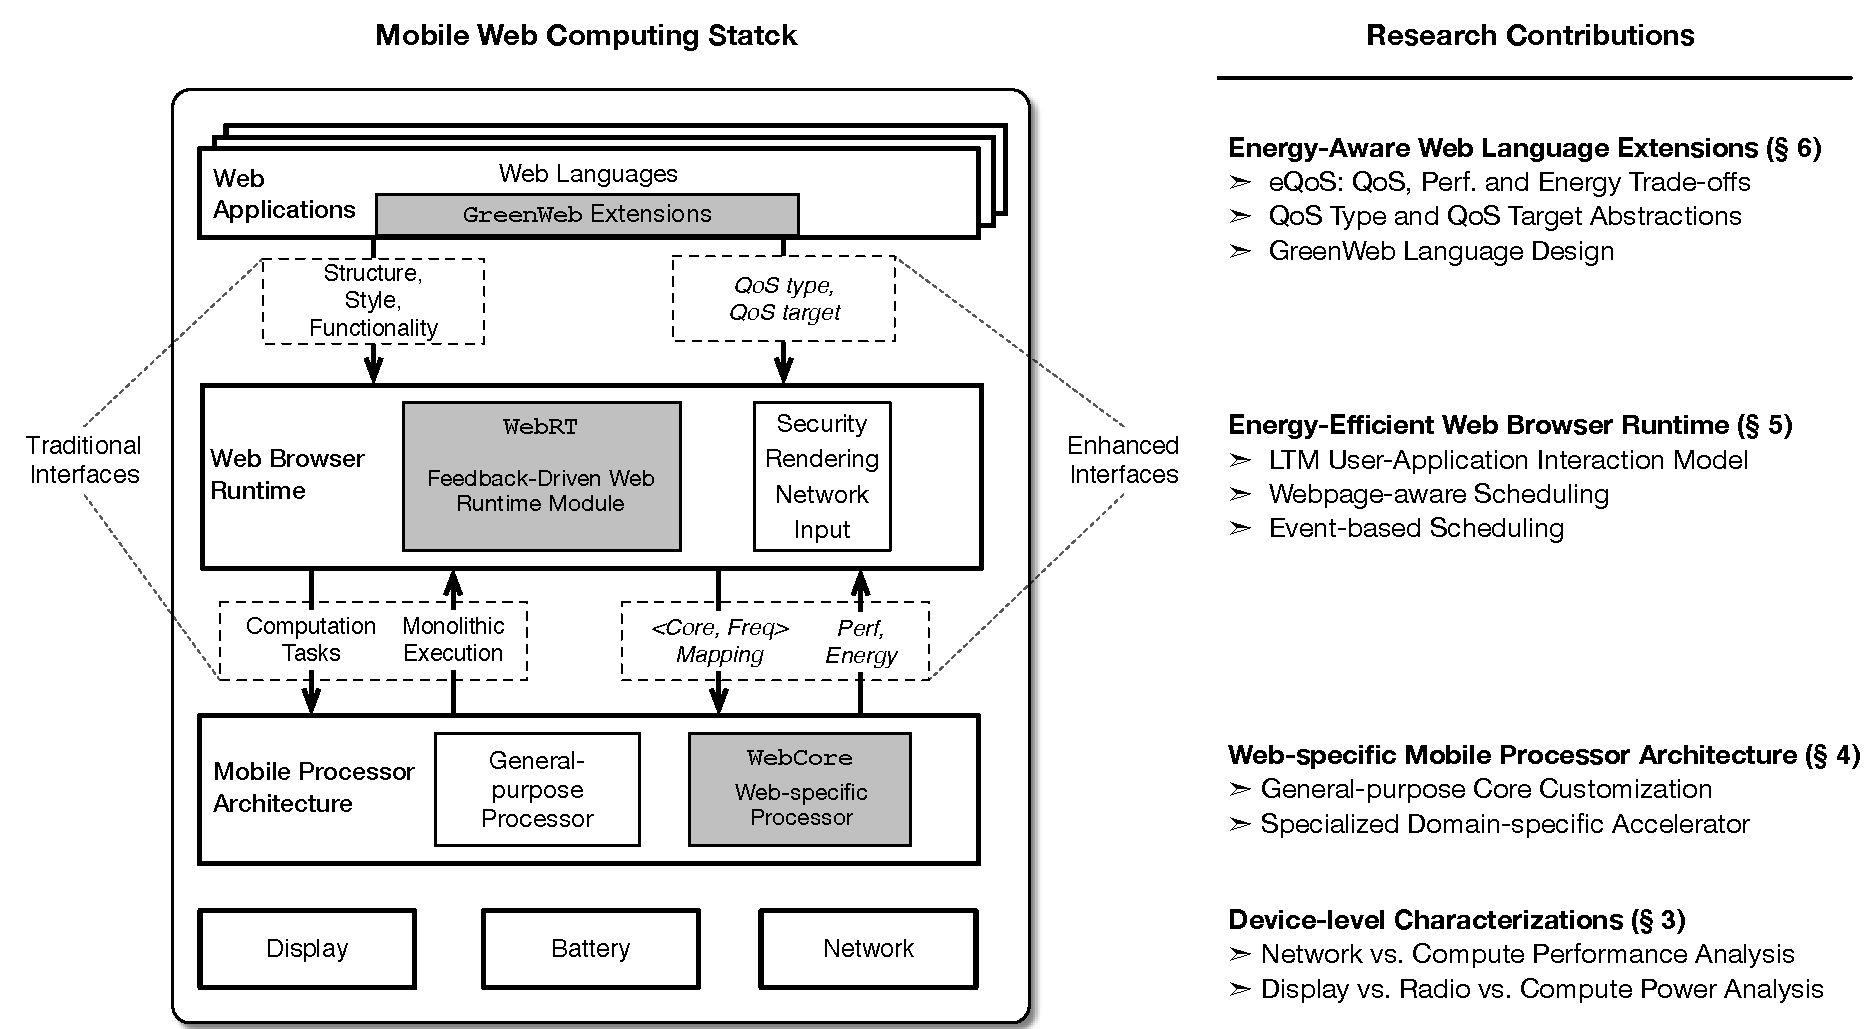
\includegraphics[trim=0 0 0 0, clip, width=\columnwidth]{framework}
  \caption{\small{Overview of the cross-layer research contributions.}}
  \label{fig:framework}
\end{figure}

I take a holistic view of the mobile Web computation stack, spanning applications, Web browser runtime, and processor architecture. Prior art has been mostly focused on optimizations within individual layers while maintaining traditional interfaces to other layers. My preliminary work~\cite{big-little, zhu2014exploiting, zhu2015role, webcore, ebs, greenweb, mobilecpu, eve-char} has demonstrated that improving energy efficiency while continuing to scale performance of the mobile Web requires us \textit{to enhance the traditional interfaces with new abstractions and to leverage the new interfaces for cross-layer optimizations}.

At the application/Web browser boundary, current Web applications merely specify visual appearance and functionalities to the browser through Web languages such as HTML, CSS, and JavaScript. User QoS requirements (e.g., latency tolerance) are unexpressed. However, different users QoS requirements lead to different optimal runtime decisions for trading off QoS with energy consumption. Exposing user QoS expectations at the application level would allow the Web runtime to budget wisely the energy usage while delivering satisfactory user QoS experience.

At the Web browser/architecture boundary, the traditional interface provides to the Web browser runtime a simple sequential execution model of the hardware.  However, today's mobile processors architectures are becoming extremely complex, combining general-purpose cores that have different performance and energy characteristics~\cite{single-ISA} with special-purpose domain-specific accelerators. While the hardware upheaval promises performance and energy improvements for the mobile Web, its practical impact depends on how effective the Web browser can leverage it. I see needs on both improving the processor architecture for the Web domain and designing an intelligent Web browser runtime that can effectively manage the hardware complexities.

In the spirit of enhancing the traditional Web computing stack interfaces and leveraging the new interfaces to optimize each layer, I propose the following research items. \Fig{fig:framework} gives an overview of the proposed cross-layer research. Enhancements to the existing Web stack are shaded.

\begin{itemize}
\item \textbf{Web Language Extensions:} I propose \greenweb, a set of language extensions that let Web developers express user QoS expectations as program annotations. \greenweb is based on two new programming abstractions, QoS type and QoS target, that capture two fundamental aspects of user QoS experience. \greenweb does not pose any constraints on specific runtime implementations but instead supports general energy optimization techniques.

\item \textbf{Smart Web Browser Runtime:} I propose \webrt, a  mobile Web browser runtime that optimizes for energy-efficiency while delivering the specified user QoS requirements. Although \webrt is a generic runtime design, as a prototype implementation, I propose to leverage the big-little architecture as the hardware substrate, which enables \webrt to tune dynamically the hardware configurations according to user QoS requirements for energy optimizations. \webrt also continuously monitors hardware execution to enable adaptive optimizations.

\item \textbf{Web-Specific Processor Architecture:} I propose \webcore, a forward-looking mobile CPU architecture customized and specialized for the Web stack. The \webcore improves performance and energy-efficiency simultaneously by integrating domain-specific hardware that exploits critical computation kernels. \webcore also maintains general-purpose programmability, which is vital to ensure its applicability to the complex Web software stack.
\end{itemize}

The \textit{long-term impact} of my proposal lies in two fundamental aspects.  First, performance and energy will continue to be the primary constraints on mobile devices as they evolve in the future (e.g., wearables and Internet-of-Things (IoT) devices). Therefore, the problem I study is likely a long-term challenge for mobile computing. Second, the Web has been and will continue to be a universal application platform because it enables application portability to tackle the notorious device fragmentation issue~\cite{fragmentation}. The proposed techniques target fundamental computations layers of Web technologies. Thus, they are likely to have long-term applicability.

The rest of the proposal is organized as follows. \Sect{sec:motivation} quantitatively demonstrates the need for high-performance and energy-efficient computation in the mobile Web. It directly motivates the research theme of my proposal. \Sect{sec:arch}, \Sect{sec:runtime}, and \Sect{sec:lang} describe the proposed \webcore, \webrt, and \greenweb at the architecture, runtime, and application layer, respectively. \Sect{sec:conc} provides a retrospective and prospective view of the proposed work. The retrospective part summarizes the principles distilled from the work so far about building an energy-efficient mobile Web computing system; the prospective part suggests next steps for generalizing the principles and outlines specific research items planned in preparing the final dissertation.
